\documentclass[tikz]{standalone}
\usetikzlibrary{calc, positioning, arrows, arrows.meta}
\usetikzlibrary{intersections}
\begin{document}
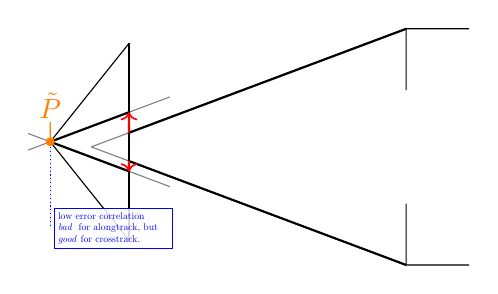
\begin{tikzpicture}

  \coordinate (pose-gt)    at (-1,  0);
  \coordinate (pose-est)   at (-1,  0.26);
  \coordinate (near-left)  at (3,  1.5);
  \coordinate (near-right) at (3, -1.5);

  \draw ($(near-left)!0.26!(near-right)$) to (near-left) to ($(near-left) + (0.8, 0)$);

  \draw ($(near-right)!0.26!(near-left)$) to (near-right) to ($(near-right) + (0.8, 0)$);

  \draw[name path=ray-left  , gray]  (pose-gt) to ($(pose-gt)!1.0!(near-left)$);
  \draw[name path=ray-right , gray] (pose-gt) to ($(pose-gt)!1.0!(near-right)$);
  % \draw[name path=ray2-left , gray]  (pose-est) to ($(pose-est)!1.0!(near-left)+(0,0.26)$);
  % \draw[name path=ray2-right, gray] (pose-est) to ($(pose-est)!1.0!(near-right)+(0,0.26)$);

  % draw lens
  \coordinate (lens-left) at ($(pose-gt)  + (1.0,  1.25)$);
  \coordinate (lens-right) at ($(pose-gt) + (1.0, -1.25)$);
  \draw[name path=lens-front, opacity=0] (lens-left) to (lens-right);

  % lens ray interections
  \fill[name intersections={of=ray-left and lens-front, name=i}] coordinate (ray-left-inter) at (i-1);
  \fill[name intersections={of=ray-right and lens-front, name=i}] coordinate (ray-right-inter) at (i-1);
  \coordinate (ray2-left-inter) at ($(ray-left-inter)+(0,0.26)$);
  \coordinate (near2-left) at ($(near-left)+(0,0.26)$);
  \coordinate (ray2-right-inter) at ($(ray-right-inter)+(0,-0.13)$);
  \coordinate (near2-right) at ($(near-right)+(0,-0.13)$);
  \coordinate (ray2-left-inter-far) at ($(near2-left)!1.6!(ray2-left-inter)$);
  \coordinate (ray2-right-inter-far) at ($(near2-right)!1.6!(ray2-right-inter)$);

  \draw[name path=ray2-left , gray] (ray2-left-inter) to (ray2-left-inter-far);
  \draw[name path=ray2-right, gray] (ray2-right-inter) to (ray2-right-inter-far);

  \fill[name intersections={of=ray2-left and ray2-right, name=i}] coordinate (pose-est) at (i-1);
  % \draw (pose-est) circle[radius=2pt];
  \coordinate (lens2-left) at ($(pose-est)  + (1.0,  1.25)$);
  \coordinate (lens2-right) at ($(pose-est) + (1.0, -1.25)$);
  \draw (pose-est) to (lens2-left);
  \draw (pose-est) to (lens2-right);
  \draw[name path=lens2-front] (lens2-left) to (lens2-right);

  \fill[name intersections={of=ray2-left and lens2-front, name=i}] coordinate (ray2-left-inter) at (i-1);
  \fill[name intersections={of=ray2-right and lens2-front, name=i}] coordinate (ray2-right-inter) at (i-1);
  \fill[name intersections={of=ray-left and lens2-front, name=i}] coordinate (ray-left2-inter) at (i-1);
  \fill[name intersections={of=ray-right and lens2-front, name=i}] coordinate (ray-right2-inter) at (i-1);

  \draw[thick] (pose-est) to (ray2-left-inter) to (ray-left2-inter) to (near-left);
  \draw[thick] (pose-est) to (ray2-right-inter) to (ray-right2-inter) to (near-right);

  \draw[->, red, semithick] (ray-left2-inter) to (ray2-left-inter);
  \draw[->, red, semithick] (ray-right2-inter) to (ray2-right-inter);



  % \draw[semithick] (pose-est) to (ray2-left-inter) to (ray-left-inter) to (near-left);
  % \draw[semithick] (pose-est) to (ray2-right-inter) to (ray-right-inter) to (near-right);


  % \draw[<->, shorten <=5, shorten >=5, blue] ($(near-left) + (0.5, 0)$) to node[fill=white] {$\Delta y\prime$} ($(near-right) + (0.5, 0)$);

  % \draw[<->, shorten <=5, shorten >=5, blue] ($(near-left) + (0.5, 0)$) to node[fill=white] {$\Delta y\prime$} ($(near-right) + (0.5, 0)$);

  \draw[orange, fill] (pose-est) circle[radius=0.05] to ++(0., +0.25) node[anchor=south, inner sep=1.0]{$\tilde{P}$};

  \draw[blue, fill, -, densely dotted, shorten <=2] (pose-est) to ++(0., -1.1) node[solid, blue, anchor=west, inner sep=4.0, outer sep=4.0, scale=0.35, draw, fill=white, fill opacity=0.85, text opacity=1]{\begin{minipage}{4cm}
      low error correlation \\
      \emph{bad\phantom{  }} for alongtrack, but \\
      \emph{good} for crosstrack.

    \end{minipage}};



\end{tikzpicture}

\end{document}
